\documentclass{article}
\usepackage{amsrefs}


\input xy
\xyoption{all}
\usepackage{enumerate}
\usepackage{pgf,tikz}
\usetikzlibrary{shapes.geometric}
\usepackage{caption}
\usepackage{subcaption}
\usetikzlibrary{matrix}
\usepackage{mathrsfs}
\usetikzlibrary{arrows}
\usepackage{stmaryrd}
\usepackage[toc,page]{appendix}


\usepackage[all,cmtip]{xy}

\usepackage{amsmath, blkarray}
\DeclareMathOperator{\res}{res}
\DeclareMathOperator{\End}{End}
\DeclareMathOperator{\im}{im}
\DeclareMathOperator{\Hom}{Hom}
\DeclareMathOperator{\Aff}{Aff}
\DeclareMathOperator{\Ext}{Ext}
\DeclareMathOperator{\rk}{rank}
\DeclareMathOperator{\Gr}{Gr}
\DeclareMathOperator{\dlog}{dlog}
\DeclareMathOperator{\coker}{coker}
\DeclareMathOperator{\Ob}{Ob}
\DeclareMathOperator{\D}{D}
\DeclareMathOperator{\Spec}{Spec}
\DeclareMathOperator{\divis}{div}
\DeclareMathOperator{\Div}{Div}
\DeclareMathOperator{\codim}{codim}
\DeclareMathOperator{\ord}{ord}
\DeclareMathOperator{\Conv}{Conv}
\DeclareMathOperator{\qis}{qis}
\DeclareMathOperator{\Int}{Int}
\DeclareMathOperator{\Pic}{Pic}
\DeclareMathOperator{\GL}{GL}
\DeclareMathOperator{\tot}{tot}
\DeclareMathOperator{\Sym}{Sym}
\DeclareMathOperator{\Cone}{Cone}
\DeclareMathOperator{\Star}{Star}
\DeclareMathOperator{\crit}{crit}
\DeclareMathOperator{\Sing}{Sing}

%Adds in a big coproduct
\let\coprod=\undefined
\DeclareSymbolFont{cmlargesymbols}{OMX}{cmex}{m}{n}
\DeclareMathSymbol{\coprod}{\mathop}{cmlargesymbols}{"60}

%Adds in a small coproduct
\let\amalg=\undefined
\DeclareSymbolFont{cmsymbols}{OMS}{cmsy}{m}{n}
\DeclareMathSymbol{\amalg}{\mathbin}{cmsymbols}{"71}



\newcommand{\Proj}{\mathbb{P}}
\newcommand{\Z}{\mathbb{Z}}
\newcommand{\C}{\mathbb{C}}
\newcommand{\calO}{\mathcal{O}}
\newcommand{\calL}{\mathcal{L}}
\newcommand{\calX}{\mathcal{X}}
\newcommand{\calE}{\mathcal{E}}
\newcommand{\calA}{\mathcal{A}}
\newcommand{\calF}{\mathcal{F}}
\newcommand{\calD}{\mathcal{D}}
\newcommand{\calH}{\mathcal{H}}
\newcommand{\calP}{\mathcal{P}}
\newcommand{\calK}{\mathcal{K}}
\newcommand{\calM}{\mathcal{M}}
\newcommand{\calC}{\mathcal{C}}
\newcommand{\calV}{\mathcal{V}}
\newcommand{\CC}{\mathbb{C}}
\newcommand{\QQ}{\mathbb{Q}}
\newcommand{\LL}{\mathbb{L}}
\newcommand{\NN}{\mathbb{N}}
\newcommand{\ZZ}{\mathbb{Z}}
\newcommand{\RR}{\mathbb{R}}
\newcommand{\VV}{\mathbb{V}}
\renewcommand{\AA}{\mathbb{A}}
\newcommand{\HH}{\mathbb{H}}
\newcommand{\PP}{\mathbb{P}}
\newcommand{\TT}{\mathbb{T}}
\newcommand{\DD}{\mathbb{D}}
\newcommand{\shO}{\mathcal{O}}
\newcommand{\shV}{\mathcal{V}}
\newcommand{\shF}{\mathcal{F}}
\newcommand{\shT}{\mathcal{T}}
\newcommand{\ra}{\to}
\newcommand {\llim}  {{\operatorname{lim}}}
\newcommand {\lra}  {\longrightarrow}
\newcommand {\id}  {\operatorname{id}}
\newcommand {\hra} {\hookrightarrow}
\newcommand {\st} {\mathrm{st}}
\newcommand {\aff} {\mathrm{aff}}
\usepackage{color}

\makeatletter
\newcommand{\xleftrightarrow}[2][]{\ext@arrow 3359\leftrightarrowfill@{#1}{#2}}
\makeatother

\newcommand{\xdasharrow}[2][->]{
% correct vertical setting by egreg:
% http://tex.stackexchange.com/a/59660/13304
\tikz[baseline=-\the\dimexpr\fontdimen22\textfont2\relax]{
\node[anchor=south,font=\scriptsize, inner ysep=1.5pt,outer xsep=2.2pt](x){#2};
\draw[shorten <=3.4pt,shorten >=3.4pt,dashed,#1](x.south west)--(x.south east);
}
}

\newcommand{\Cdot}{\boldsymbol{\cdot}}
%\newcommand{\defeq}{\mathrel{\mathop:}=}
\newcommand{\eqdef}{\mathrel{\mathop=}:}

\newcommand*{\defeq}{\stackrel{\text{def}}{=}}

\usepackage{amsmath,amsfonts,mathdots,epstopdf}
\usepackage{amsmath, amsthm, amssymb, amsfonts, mathrsfs}
\usepackage{thmtools}
\usepackage{graphicx}
\graphicspath{ {./images/} }
\usepackage{setspace}
\usepackage{geometry}
\usepackage{float}
\usepackage{hyperref}
\usepackage[utf8]{inputenc}
\usepackage[english]{babel}
\usepackage{framed}
\usepackage[dvipsnames]{xcolor}
\usepackage{tcolorbox}
\usepackage{tikz-cd}
\usepackage{epigraph}


\colorlet{LightGray}{White!90!Periwinkle}
\colorlet{LightOrange}{Orange!15}
\colorlet{LightGreen}{Green!15}
\definecolor{powderblue(web)}{rgb}{0.69, 0.88, 0.9}


\newcommand{\HRule}[1]{\rule{\linewidth}{#1}}

\declaretheoremstyle[name=Theorem,]{thmsty}
\declaretheorem[style=thmsty,numberwithin=subsection]{theorem}
\tcolorboxenvironment{theorem}{colback=LightOrange}

\declaretheoremstyle[name=Proposition,]{prosty}
\declaretheorem[style=prosty,numberlike=theorem]{proposition}
\tcolorboxenvironment{proposition}{colback=LightGreen}

\declaretheoremstyle[name=Lemma,]{lemsty}
\declaretheorem[style=lemsty,numberlike=theorem]{lemma}
\tcolorboxenvironment{lemma}{colback=LightGray}

\tcolorboxenvironment{lemdef}{colback=LightGray}

\tcolorboxenvironment{cor}{colback=powderblue(web)}



\newtheorem{thm}{Theorem}
\newtheorem{prop}{Proposition}
\newtheorem{defn}[theorem]{Definition}
\newtheorem{conv}{Convention}
\newtheorem{rem}{Remark}
\newtheorem{lem}{Lemma}
\newtheorem{lemdef}[theorem]{Lemma/Definition}
\newtheorem{cor}[theorem]{Corollary}
\newtheorem{nota}{Note}
\newtheorem{es}{Example}[subsection]
\newtheorem{fact}{Fact}
\newtheorem{ex}{Exercise}
\numberwithin{equation}{section}

\setstretch{1.2}
\geometry{
 textheight=9in,
  textwidth=5.5in,
  top=1in,
  headheight=12pt,
  headsep=25pt,
  footskip=30pt
}


%\geometry{a4paper,top=3.5cm,bottom=3.5cm,left=2.5cm,right=2cm}



%\newcommand{\verteq}[0]{\begin{turn}{90} $=$\end{turn}}

% ------------------------------------------------------------------------------
\setcounter{section}{-1}
\usepackage{subfiles} % Best loaded last in the preamble

% ------------------------------------------------------------------------------

\title{Mixed Hodge Structures and Mirror Symmetry}
\author{Edoardo Manini}
\date{ }

\begin{document}
\newgeometry{top=2cm,bottom=2cm,left=2.5cm,right=2cm}
\begin{titlepage}
    \begin{center}
        
\includegraphics[height=5cm]{tesiSCIENZE_TECNOLOGIE.jpg}
        \vspace*{0.5cm}

        \LARGE

        \textbf{Corso di Laurea Magistrale in Matematica}

        \vspace*{2cm}
        
        \huge
        \textsc{Mixed Hodge Structures and\\}
        \textsc{Mirror Symmetry}

        \normalsize
        \vspace*{4cm}

        \begin{minipage}[t]{0.47\textwidth}
	       {\large {Relatore:}} \vspace{0.3em} \\
              {\large {Prof. Diego MATESSI}} \vspace{1em} \\
	       {\large {Correlatore:}} \vspace{0.3em} \\
              {\large {Prof. Luigi LOMBARDI}} \vspace{1em}
        \end{minipage}
        \hfill
        \begin{minipage}[t]{0.47\textwidth}\raggedleft
	       {\large {Candidato:}} \hspace{-0.9em} \vspace{0.3em} \\
              {\large {Edoardo Manini}} \\
               {\large Matricola: 27724A}
        \end{minipage}

        \vfill
        \large Anno Accademico 2023/2024
            
    \end{center}
\end{titlepage}






\newpage
\thispagestyle{empty}
\mbox{}
\newpage

%\begin{titlepage}
    %\vspace*{5cm} % Regola questo valore per %posizionare il testo verticalmente
   % \begin{flushright}
        %{\large % Puoi modificare le dimensioni del %testo
  %      \textit{Ai miei genitori.}
 %       }
%    \end{flushright}
%\end{titlepage}
\restoregeometry
\tableofcontents
\pagebreak


%Vecchia impostazione
%\maketitle
%\newpage
%\tableofcontents
%\newpage

% ------------------------------------------------------------------------------



\section{Introduction}
The main goal of this thesis is to study mixed Hodge theory and apply its tools to an extension of classical Mirror Symmetry, originally formulated for pairs of Calabi-Yau manifolds, to a broader class of varieties. In particular, following \cite{GKR17}, we study a construction of a mirror dual for a genus 2 curve and we calculate the Hodge numbers of the mirror using the monodromy weight spectral sequence associated to the cohomological mixed Hodge complex structure on the sheaf of vanishing cycles.

The employment of mixed Hodge structures is necessary since the varieties in the construction of non-Calabi Yau mirror symmetry are in general not smooth.
For this reason we spend a great deal of time studying mixed Hodge structures extensively.

The structure of the thesis is as follows.
The first two chapters contain a summary of classical Hodge theory, Hodge structures and their variations.
The third chapter introduces the notion of mixed Hodge structure, central for extending features of classical Hodge theory to not necessarily compact K\"{a}hler (projective) varieties. The next chapter deals with families of varieties degenerating to a singular variety. Finally, the last two chapters treat two particular constructions in the mathematical side of Mirror Symmetry, a theory which originates from particle physics. 

%
%Chapter one
%

Hodge theory is a vast area of study in complex algebraic geometry. 
Firstly we illustrate classical results which form the foundation of Hodge theory like Hodge's theorem, the isomorphism between the space of harmonic differential $k$-forms and the $k$-th cohomology group on a compact oriented Riemannian manifold. Then, restricting our attention to K\"{a}hler manifolds, one proves the Hodge identities which imply that the $d$, $\partial$ and $\bar \partial$-Laplacians are proportional to each other, which in turn implies that the $d$-Laplacian respects the bidegree. From this, it immediately follows a decomposition of the space of harmonic forms that in the compact K\"{a}hler case gives the famous Hodge decomposition and Hodge symmetry theorems. 
\begin{align}
        H^k(X,\CC) &= \bigoplus_{p+q=k} H^{p,q}(X) \label{eq:eq1}\tag{Hodge Decomposition} \\
        H^{p,q}(X) &= \overline{H^{q,p}(X)} \label{eq:eq2}\tag{Hodge Symmetry}
\end{align}
This decomposition, among many consequences, gives a topological constraint for compact K\"{a}hler manifolds: their odd Betti numbers are even. Hodge numbers are usually displayed inside the Hodge diamond. We work out some examples of such diamonds. The main reference here is \cite{Voi07}.


\begin{figure}[ht]
  \begin{subfigure}[b]{0.3\textwidth}
    \centering 
\begin{tikzpicture}[scale=1]
\draw (0.5,0) node              {$g$};
\draw (-0.5,0) node             {$g$};
\draw (0,0.5) node              {$1$};
\draw (0,-0.5) node             {$1$};
\draw (1,0) -- (0,1) -- (-1,0) -- (0, -1) -- cycle;
\end{tikzpicture}
    \caption{genus $g$ curve}
    \label{genusGdiamond}
  \end{subfigure}
  \hfill
  \begin{subfigure}[b]{0.3\textwidth}
  \centering
\begin{tikzpicture}[scale=1]
\draw (1,0) node              {$1$};
\draw (-1,0) node             {$1$};
\draw (0.5,0.5) node              {$0$};
\draw (-0.5,0.5) node             {$0$};
\draw (0,0) node              {$20$};
\draw (0.5,-0.5) node              {$0$};
\draw (-0.5,-0.5) node             {$0$};
\draw (0,1) node              {$1$};
\draw (0,-1) node             {$1$};
\draw (1.5,0) -- (0,1.5) -- (-1.5,0) -- (0, -1.5) -- cycle;
\end{tikzpicture}
    \caption{K3 surface}
    \label{K3_diamond}
  \end{subfigure}
  \hfill
  \begin{subfigure}[b]{0.3\textwidth}
 \centering 
\begin{tikzpicture}[scale=1]
\draw (1.5,0) node              {$1$};
\draw (-1.5,0) node             {$1$};
\draw (0.5,0) node              {$101$};
\draw (-0.5,0) node             {$101$};
\draw (1,0.5) node             {$0$};
\draw (0,0.5) node              {$1$};
\draw (-1,0.5) node             {$0$};
\draw (1,-0.5) node             {$0$};
\draw (0,-0.5) node              {$1$};
\draw (-1,-0.5) node             {$0$};
\draw (0.5,1) node              {$0$};
\draw (-0.5,1) node             {$0$};
\draw (0.5,-1) node              {$0$};
\draw (-0.5,-1) node             {$0$};
\draw (0,1.5) node              {$1$};
\draw (0,-1.5) node             {$1$};
\draw (2,0) -- (0,2) -- (-2,0) -- (0, -2) -- cycle;
\end{tikzpicture}
    \caption{quintic threefold}
    \label{quintic_diamond}
  \end{subfigure}
  \caption{some Hodge diamonds}
\end{figure}

%Cup product with the $(1,1)$-K\"{a}hler form gives the Lefschetz map which gives a further decomposition, the Lefschetz decomposition.
The structure on the $k$-th cohomology of a compact K\"{a}hler manifold $X$ is a Hodge structure of weight $k$. This means we have a lattice $H_\ZZ$, here $H^k(X,\ZZ) / \textrm{torsion}$, together with a decomposition of its complexification $H_\CC = \bigoplus_{p+q=k} H^{p,q}$ satisfying $H^{p,q} = \overline{H^{q,p}}$. To give a Hodge structure of weight $k$ on $H_\ZZ$ is equivalent to give a decreasing filtration $\{ F^p \}$ on $H_\CC$ satisfying $F^p \oplus \overline{F^{k-p+1}} \simeq H_\CC$. A filtration with this property is called a \emph{Hodge filtration}.
There are many ways of constructing new Hodge structures from given ones and moreover they form an abelian category. The introduction of a polarization, together with the Hodge-Riemann bilinear relations allows to study a classification of polarized Hodge structures as points in a moduli space called local period domain.

%
%Chapter two
%

The second chapter introduces the study of families of compact K\"{a}hler manifolds and the concepts of a polarized variation of Hodge structure and of the period map associated to it. The references for this part are \cite{FRT15}, \cite{CMSP03} and \cite{Voi07}. The Hodge subspaces of the cohomology of the fibres of a family may vary, nevertheless their dimensions remain fixed. The local period domains have structures of algebraic (flag) varieties. We see some examples. When the base space of the family is not simply connected, we need to quotient the period domain by a monodromy group in order to have a well defined global period map.
This is known as the geometric setting. Abstract variations of Hodge structure is a generalization of this case. The Leray sheaves are substituted by any local system on the base manifold and the Gauss-Manin connection is replaced by a flat connection satisfying Griffiths transversality.


%
%Chapter three
%

Deligne established the existence of a linear algebraic structure on the cohomology of complex algebraic varieties, called mixed Hodge structure; it reflects geometric and topological properties of algebraic varieties, which means it depends on the geometry and not only the topology of such varieties. This theory is analyzed thoroughly in the third chapter. The main reference here is \cite{PS08}.
A \emph{mixed Hodge structure} is the data of $(H_\ZZ,W,F)$ where $H_\ZZ$ is a free f.g. $\ZZ$-module, $W$ a finite increasing filtration on the rational vector space $H_\QQ = H \otimes \QQ$:
\[
{0}\subset\cdots\subset W_0\subset W_1\subset W_2\subset \cdots\subset H_\QQ
\] 
called \emph{weight filtration} and $F$ is a finite decreasing filtration on $H_\CC =H \otimes \CC$:
\[
H_{\CC} =F^0\supset F^{1}\supset F^2\supset\cdots\supset{0}
\] 
called \emph{Hodge filtration}, such that the induced filtration by $F$ on the graded piece $\Gr^W_k H_\CC=W_{k}H_\CC/W_{k-1}H_\CC$ defines a pure Hodge structure of weight $k$.
%Morphisms of MHS preserve by definition both filtrations and can be shown to be strict, which implies that an injection of MHS is still an injection when considered as the induced map on graded pieces. For this reason, mixed Hodge structures respect exact sequences.
The main theorem of Deligne of mixed Hodge theory states that for every complex algebraic variety, the integral cohomology groups carry a natural mixed Hodge structure, functorial with respect to algebraic maps.
We give the construction of the MHS in the case of a not necessarily compact smooth algebraic variety $U$. By Nagata embedding theorem, $U$ is Zariski open in some compact algebraic variety $X$, which by Hironaka, we can choose to be smooth and s.t. $D=X \setminus U$ is a normal crossing divisor (NCD) in $X$. To take into account the properties of the NCD, we need to introduce the logarithmic de Rham complex $\Omega^\bullet_X ( \log D)$ of forms having poles of order at most one along $D$. Deligne showed that this complex is quasi-isomorphic to (the pushforward of) the De Rham complex of $U$, which implies that its hypercohomology is the cohomology of the variety $U$. To construct the MHS then, it suffices to construct two filtrations $W,F$ on the logarithmic De Rham complex, the first one by order of poles and for the second one we take the naive one and verify that they satisfy some properties so that the induced filtrations in hypercohomology induce a mixed Hodge structure on $H^n(U)$. These properties are encoded in the definition of a mixed Hodge complex of sheaves. After seeing some concrete examples of this construction we extrapolate the properties and come to the axioms of mixed Hodge complexes and (cohomological) mixed Hodge complexes of sheaves.
The construction of the \emph{mixed cone} for a morphism of mixed Hodge complexes of sheaves allows us to get induced long exact sequences of MHS's. Moreover one can define mixed Hodge structures on relative cohomology groups. In an example, we calculate the Hodge numbers and the long exact sequence of the pair. Finally, we see another important example of a mixed Hodge structure, namely the one on the cohomology of a singular normal crossing variety, which is defined via a cohomological mixed Hodge complex $B^\bullet$. We carry out calculations in the example of three lines in $\PP^2$, i.e. the normal crossing variety $V(xyz) \subset \PP^2$, topologically a necklace of three spheres.

%
%Chapter four
%

In chapter four we investigate what happens near a singular fiber of a degenerating family. In particular we are interested in $1$-parameter semistable degenerations, i.e. proper holomorphic maps $f \colon X \to \Delta$ over the unit disk that are smooth away from a reduced simple normal crossing central fibre $Y = f^{-1}(0)$. The main references here are \cite{Sc73} and \cite{PS08}.
Some of the tools needed to study them are connections with logarithmic poles and their residues. The reason being that the cohomology of the smooth fibres over the punctured disk $\Delta^* = \Delta \setminus \{0 \}$ form local systems equipped with a flat connection that acquires a logarithmic singularity and its residue is related to the monodromy automorphism $T$ around the singular fibre. $T$ is quasi-unipotent, i.e. there exists positive integers $l,m \in \NN$ s.t. $(T^l - \id)^{m}=0$. This is the content of the monodromy theorem proved by Schmid. The logarithm of the unipotent part of the monodromy $N$ is then a nilpotent endomorphism. A linear algebra lemma says that whenever we have a nilpotent endomorphism on a finite dimensional vector space, we have an associated increasing filtration $W(N)$ which is unique satisfying certain properties. In 1973, Schmid used this monodromy weight filtration together with a limiting filtration $F_{\lim}$ to define the so called \emph{limiting mixed Hodge structure}. In the case of a semistable degeneration, this limiting MHS is induced by a cohomological mixed Hodge complex (CMHC) on the sheaf of nearby cocycles $\psi_f \CC_X$ which is a sheaf on the singular fibre. Its (hyper-)cohomology is isomorphic to the cohomology of the nearby smooth fibre. Section 4.5 %\ref{Sect.CMHC.LMHS}
is dedicated to this CMHC. Its construction starts with a double complex whose total complex $A^\bullet$ we show to be quasi-isomorphic to the relative De Rham complex which is itself quasi-isomorphic to the sheaf of nearby cocycles. The degeneracy at the second page of the monodromy weight spectral sequence and the computation of the differentials in the first page allow us to read Hodge numbers off of the $E_2$-page. We conclude with Steenbrink long exact sequence of MHS induced by a short exact sequence of CMHC's relating $B^\bullet$ and $A^\bullet$:
\[
0 \lra B^\bullet \xrightarrow{\mathrm{sp}} A^\bullet \lra \bar A^\bullet \lra 0
\]
where $\bar A^\bullet$ is isomorphic to the sheaf of vanishing cycles $\phi_f \CC_X$. We end the chapter showing this theory within an example of a family of elliptic curves degenerating to a singular central fibre.

%
%Chapter five
%

In the final part of the thesis we study the application of this theory to Mirror Symmetry.
Superstring theory suggests that there are six extra dimensions of spacetime in addition to the four of Einstein. Moreover these six (real) dimension must be shaped like a (complex) three-dimensional Calabi-Yau manifold. Additionally, theoretical physicists discovered a duality for Calabi-Yau $3$-folds which is called Mirror Symmetry. This correspondence, among other things, implies a duality of Hodge numbers between the two mirror partners. 
If two smooth $n$-dimensional Calabi-Yau manifolds $Y$ and $Y^\circ$ are mirror partners, then
\begin{align} \label{MirrorSymmetry}
 h^{p,q}(Y) = h^{n-p,q}(Y^\circ) \quad \text{ for } \quad  0 \leq p,q \leq n.
\end{align}
The main references for this part are \cite{CK99} and \cite{CLS11}.
In chapter five we review the construction of Batyrev of mirror pairs of CY's, which makes use of toric geometry. From a reflexive polytope $\Delta$, one derives a Fano variety $X_\Delta$. It is the toric projective variety associated to the normal fan $\Sigma_\Delta$ of the polytope. Every reflexive polytope $\Delta$ has a polar dual $\Delta^\circ$ which is also reflexive and this duality lifts to a duality between families of Calabi-Yau hypersurfaces in certain toric varieties closely related to $X_\Delta$ and $X_{\Delta^\circ}$. Letting $Y^\circ$ be the so called \emph{Batyrev mirror} of $Y$, and $n=\dim Y = \dim Y^\circ$, then 
\[
h^{1,1}(Y) = h^{n-1,1}(Y^\circ) \quad \text{ and } \quad  h^{n-1,1}(Y) = h^{1,1}(Y^\circ).
\]
For a threefold, $n=3$, this is all is needed to prove the duality of Hodge diamonds \eqref{MirrorSymmetry}.
The last chapter is dedicated to the construction of \cite{GKR17}, where a mirror duality is proposed for pairs of Landau-Ginzburg models $(X,w) \leftrightarrow (\check{X}, \check{w})$, i.e. quasi-projective varieties with non-constant regular functions.    
Here, we witness the interplay between mixed Hodge structures and Mirror Symmetry. Indeed, the mirror of a smooth not necessarily Calabi-Yau variety $\check{S}$ is a possibly singular variety $S$ which needs to be furnished with the sheaf of vanishing cycle (shifted by one) $\calF_S$. Once we define Hodge numbers for the pair $(S,\calF_S)$, the main theorem is 
\[
h^{p,q}(\check{S})= h^{d-p,q}(S,\calF_S),
\]
where $d=\dim S = \dim \check{S}$.
Here the construction also involves toric geometry but we don't restrict ourselves to reflexive polytopes. The mirror of a genus $2$ curve turns out to be topologically a configuration of three projective lines intersecting in two triple points. See figure \ref{genus2mirror} below.
\begin{figure}[ht!]
\centering
    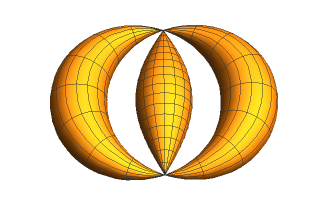
\includegraphics[width=8cm]{images/Genus_2_Mirror.png}
    \caption{Mirror of a genus 2 curve}
    \label{genus2mirror}
\end{figure}
We carry out calculations of Hodge numbers for the mirror of a genus $2$ curve verifying the Mirror theorem.  To do so, we employ the monodromy weight spectral sequence for the sheaf of vanishing cycles we saw before. We see in this example that the Hodge diamond of the mirror dual of a genus $2$ curve is the one of a genus $2$ curve, mirrored along the \emph{mirror axis}, the $45^\circ$ line through the center of the diamond.

\begin{figure}[ht]
  \begin{subfigure}[b]{0.4\textwidth}
    \centering 
\begin{tikzpicture}[scale=1]
\draw (0.5,0) node              {$2$};
\draw (-0.5,0) node             {$2$};
\draw (0,0.5) node              {$1$};
\draw (0,-0.5) node             {$1$};
\draw (1,0) -- (0,1) -- (-1,0) -- (0, -1) -- cycle;
\end{tikzpicture}
    \label{S_check_Hodge_diamond}
  \end{subfigure}
  \hfill
  \begin{subfigure}[b]{0.4\textwidth}
 \centering 
\begin{tikzpicture}[scale=1]

\draw (0.5,0) node              {$1$};
\draw (-0.5,0) node             {$1$};
\draw (0,0.5) node              {$2$};
\draw (0,-0.5) node             {$2$};
\draw (1,0) -- (0,1) -- (-1,0) -- (0, -1) -- cycle;
\end{tikzpicture}
    \label{ScalF_S_diamond}
  \end{subfigure}
  \caption{Hodge diamonds of a genus 2 curve and its mirror}
\end{figure}




\section{Hodge Theory}
\subfile{sections/HodgeTheory}

\section{Variations of Hodge Structure}\label{sect:vhs}
\subfile{sections/variations}


\section{Mixed Hodge Structures}\label{sect:mhs}
\subfile{sections/MHS}


\section{Degenerations of Hodge Structures}
\subfile{sections/degenerations}


\section{Mirror Symmetry for Calabi-Yau varieties}
\subfile{sections/MSCY}


\section{Mirror symmetry for Landau-Ginzburg models}
\subfile{sections/MSLG}


\newpage

\begin{appendices}

\section{Spectral Sequences}\label{SpSeq}
\subfile{sections/SpSeq}


%\section{Exact categories and Abelian categories}\label{ExAb}

%\subsection{Derived categories}\label{DerCat}



\end{appendices}


\bibliographystyle{apalike} 
\begin{thebibliography}{70}


\bibitem[Bat94]{Bat94}
V. Batyrev, \emph{Dual Polyhedra and Mirror Symmetry for Calabi-Yau Hypersurfaces in Toric Varieties}, J. Algebraic Geom. 3, p.493–535, 1994.



\bibitem[BB94]{BB94}
V. Batyrev, and L. Borisov,  \emph{On Calabi-Yau complete intersections in toric varieties}, in Higher Dimensional Complex Varieties: Proceedings of the International Conference held in Trento, Italy, June 15 - 24, 1994, Berlin, New York: De Gruyter, pp. 39-66, 1996.


\bibitem[BB96]{BB96}
V. Batyrev, L. Borisov, \emph{Mirror duality and string-theoretic Hodge numbers}, Invent math 126, 183–203, 1996.


\bibitem[BHPV04]{BHPV04}
W.~P. Barth, K.~Hulek, C.~A.~M. Peters, and A.~van~de Ven, \emph{Compact
  complex surfaces}, second ed., Ergebnisse der Mathematik und ihrer
  Grenzgebiete, 3. Fogle, A Series of Modern Surveys in Mathematics, vol.~4,
  Springer-Verlag, 2004.


\bibitem[COGP91]{COGP91}
P. Candelas, X.C. de la Ossa, P.S. Green, and L. Parkes, 
\emph{A pair of Calabi-Yau manifolds as an exactly soluble superconformal theory}, Nuclear Phys. B 359, 21-74, 1991.
  
\bibitem[CMSP03]{CMSP03}
J.~Carlson, S.~M{\"u}ller-Stach, and C.~A.~M. Peters, \emph{Period mappings and
  period domains}, Cambridge Studies in Advanced Mathematics, vol.~85,
  Cambridge University Press, 2003.



\bibitem[CLS11]{CLS11}
D. A. Cox, J. B. Little, and H. K. Schenck, \emph{Toric varieties}, volume 124 of Graduate Studies in Mathematics, American Mathematical Society, United States, 2011.

  
\bibitem[CK99]{CK99}
D.~A. Cox, and S.~Katz, 
\emph{Mirror Symmetry and Algebraic Geometry},
  Mathematical surveys and monographs,
  American Mathematical Society, 1999.


\bibitem[Cl77]{Cl77}
C.~H. Clemens, \emph{Degeneration of {K}{\"a}hler manifolds}, Duke Math. J.
  \textbf{44}, no.~2, 215--290, 1977.


\bibitem[Cl80]{Cl80}  
C.~H. Clemens, \emph{A Scrapbook of Complex Curve Theory}, Plenum University Press, New York, London, 1980.


\bibitem[Cl84]{Cl84} 
C.~H. Clemens, \emph{Some results about Abel-Jacobi mappings}, Topics in transcendental algebraic geometry (Princeton, N.J., 1981/1982), 289–304. Ann. of Math. Stud., 106 Princeton University Press, Princeton, NJ, 1984.


\bibitem[DK86]{DK86} 
V.I. Danilov, A.G. Khovanskii, \emph{Newton polyhedra and an algorithm for computing Hodge-Deligne numbers}, Izv. Akad. Nauk SSSR Ser. Mat. 50:5, p.925–9, 1986.


\bibitem[Del70]{Del70}
P.~Deligne, \emph{Equations diff{\'{e}}rentielles {\'{a}} points singuliers r{\'{e}}guliers}, Springer Lecture Notes in Math., 163, 1970.


  
\bibitem[Del71]{Del71}
\bysame, \emph{Th{\'{e}}orie de {H}odge {II}}, Inst. Hautes {\'E}tudes Sci. Publ. Math., no.~40, 5--57, 1971.

  
\bibitem[Del74]{Del74}
\bysame, \emph{Th{\'{e}}orie de {H}odge {III}}, Inst. Hautes {\'E}tudes Sci. Publ. Math. no.~44, 5--77, 1974.


\bibitem[Del10]{Del10}
\bysame, \emph{Le thèoréme de plongement de Nagata}, Kyoto Journal of Mathematics 50, 2010.


\bibitem[FRT15]{FRT15}
S. Filippini , H. Ruddat, A. Thompson ,
   \emph{An Introduction to Hodge Structures}, Calabi-Yau Varieties: Arithmetic, Geometry and Physics, Springer New York, 83–130, 2015. 


\bibitem[Ful93]{Ful93}
  W. Fulton. \emph{Introduction to Toric Varieties}, (AM-131), Volume 131. Princeton University
Press, Princeton, 1993.

\bibitem[Gr70]{Gr70}
P. Griffiths, \emph{Periods of integrals on algebraic manifolds: Summary of main
  results and discussion of open problems}, Bull. Amer. Math. Soc. \textbf{76},  228--296, 1970.


\bibitem[GHJ03]{GHJ03}
M. Gross, D. Huybrechts, and D. Joyce, \emph{Calabi-Yau Manifolds and Related Geometries}, Springer, Universitext, 2003.


\bibitem[Gi96]{Gi96}
 A. Givental \emph{Equivariant Gromov-Witten invariants}, Internat. Math. Res. Notices , no. 13, 613–663, 1996.


\bibitem[Gi98]{Gi98}
\bysame, \emph{A mirror theorem for toric complete intersevections}, in Topological field theory, primitive forms and related topics (Kyoto, 1996), Progr. Math., 160, Birkhauser Boston, MA, p.141–175, 1998.


\bibitem[GKR17]{GKR17}
 M.~Gross, L.~Katzarkov, H.~Ruddat, \emph{Towards Mirror Symmetry for Varieties of General Type}, Advances in Mathematics, 308, 208-275, 2017.

\bibitem[Groth66]{Groth66}
 A. Grothendieck, \emph{On the de Rham cohomology of algebraic varieties}, Publ. Math. IHES, 29: 95–103, 1966.


\bibitem[Har77]{Har77}
R. Hartshorne, \emph{Algebraic Geometry}, Graduate Texts in Math. 52, Springer, New York, 1977.


\bibitem[Hel64]{Hel64}
S. Helgason, \emph{Differential Geometry and Symmetric Spaces}, American Mathematical Society, 1964.


\bibitem[Iver86]{Iver86}
B. Iversen, \emph{Cohomology of sheaves}. Universitext, Springer-Verlag, Berlin, 1986.


\bibitem[Katz86]{Katz86}
 S. Katz, \emph{On the finitness of rational curves on quintic threefolds}, Compositio Math. 60, 151-162, 1986.

\bibitem[KO68]{KO68} 
S. Katz, N. Oda, \emph{On the differentiation of the De Rham cohomology classes with respect to parameters}, J. Math. Kyoto Univ.1, 199–213, 1968.

\bibitem[Kon95]{Kon95}
M. Kontsevich, \emph{Homological Algebra of Mirror Symmetry}, In: Chatterji, S.D. (eds) Proceedings of the International Congress of Mathematicians. Birkhäuser, Basel, 1995.


\bibitem[Ku98]{Ku98}
V.~Kulikov, \emph{Mixed {H}odge structures and singularities}, Cambridge Tracts
  in Mathematics, vol. 132, Cambridge University Press, 1998.


\bibitem[OdP91]{OdP91}
T.Oda, H. S. Park, \emph{Linear Gale transforms and Gelfand-Kapranov-Zelevinskij decompositions}, Tohoku Math. J. (2) 43 (3) 375 - 399, 1991.

\bibitem[PS08]{PS08}
C.~A.~M. Peters and J.~H.~M. Steenbrink, \emph{Mixed {H}odge structures},
  Ergebnisse der Mathematik und ihrer Grenzgebiete, 3. Fogle, A Series of
  Modern Surveys in Mathematics, vol.~52, Springer, 2008.


\bibitem[Reid87]{Reid87}
   M. Reid, \emph{Young person’s guide to canonical singularities}, in Algebraic Geometry, Bowdoin 1985, ed. S. Bloch, Proc. of Symposia in Pure Math. 46, A.M.S., vol. 1, 345–414, 1987.

  
\bibitem[Sc73]{Sc73}
W.~Schmid, \emph{Variation of {H}odge structure: The singularities of the
  period mapping}, Invent. Math. \textbf{22} (1973), 211--319.



\bibitem[St75]{St75}
J.~H.~M. Steenbrink, \emph{Limits of {H}odge structures}, Invent. Math.
  \textbf{31} (1975), no.~3, 229--257.


\bibitem[St77]{St77}
\bysame, \emph{Mixed Hodge structures on the vanishing cohomology}, in Real and Complex Singularities, Oslo, 1976, Sijthoff-Noordhoff, Alphen a/d Rijn, 525–563, 1977.



\bibitem[Thu97]{Thu97}
 W. Thurston, \emph{The Geometry and Topology of Three-Manifolds}, Princeton University Press, 1997.
 

\bibitem[Voi07]{Voi07}
C.~Voisin, \emph{{H}odge theory and complex algebraic geometry. {I}}, Cambridge
  Studies in Advanced Mathematics, vol.~76, Cambridge University Press, 2007.

\bibitem[Wlo05]{Wlo05}
J. Wlodarczyk, \emph{Simple Hironaka resolution in characteristic zero}, Journal of the American Mathematical Society 18, Oct. 2005.

\end{thebibliography}



\newpage
\thispagestyle{empty}
\mbox{}
\newpage

\section*{Ringraziamenti}
Voglio ringraziare il prof. Matessi per avermi proposto gli argomenti di questa tesi e per avermi seguito nel loro studio, dandomi preziosi consigli.

Ringrazio i miei genitori per il loro fondamentale costante supporto durante questi $3+2$ ($+20$) anni. 
Ringrazio mia sorella Sara per essere sempre al mio fianco. 
Ringrazio tutti i miei amici per il vostro affetto e sostegno. 
Gli ex-compagni del liceo, gli amici del mare e i `` colleghi '' dell'università. \'E grazie anche a tutte le esperienze passate insieme che sono arrivato alla fine di questo percorso. 
Grazie Fabio per avermi accompagnato nell'avventura di Bonn, porterò sempre con me la tua gentilezza. 
Grazie Flavio per le nostre discussioni sulla geometria torica.
Grazie Cosimo e Federico perchè riuscite sempre a farmi ridere.
Poi voglio ringraziare i miei nonni per il loro infinito amore.
Infine dico grazie a te Eleonora, per troppi motivi che il margine di questa pagina non può contenere. Grazie che ci sei e mi sei sempre vicino pur nei miei numerosi difetti. 



\end{document}